\documentclass{article}
\usepackage{ctex}
\usepackage{makecell}
\usepackage{graphicx}
\usepackage{geometry}
\usepackage{multirow}
\usepackage{multicol}
\usepackage{fancyhdr}
\usepackage{longtable}
\usepackage{color}
\usepackage{float}
\usepackage{listings}
\usepackage{xcolor}
\usepackage{hyperref}
\usepackage{footnote}
\usepackage{paralist}
\usepackage{amsmath}
\usepackage{subcaption}

\newcommand{\tabitem}{~~\llap{\textbullet}~~}
\renewcommand{\labelitemii}{\textbullet}
\renewcommand{\labelitemiii}{\textbullet}

\let\itemize\compactitem
\let\enditemize\endcompactitem
\let\enumerate\compactenum
\let\endenumerate\endcompactenum
\let\description\compactdesc
\let\enddescription\endcompactdesc

\geometry{a4paper,left=25mm,right=20mm,top=25mm,bottom=25mm}

\title{我对AI算法在图像处理中应用的原理理解和未来展望}
\author{09021227~金桥}
\date{\today}

\lstset{
    numbers=left,
    keywordstyle= \color{ blue!70},
    commentstyle= \color{red!50!green!50!blue!50},
    rulesepcolor= \color{ red!20!green!20!blue!20} ,
    % escapeinside=``,
    numberstyle=\tt,
    numbersep=0em,
    xleftmargin=2em,
    breaklines,
    aboveskip=1em,
    framexleftmargin=2em,
    frame=shadowbox,
    basicstyle=\tt,
    language=C++
}

\begin{document}

\maketitle


人工智能(AI)已经在各种领域中发挥了重要作用,其中图像处理是最具影响力的应用之一。从医疗影像分析到自动驾驶,从计算机视觉到增强现实,AI在图像处理中的应用广泛且深入。本报告将探讨AI在图像处理中的原理,并对未来的发展趋势进行展望。

\section{AI在图像处理中的原理}

\subsection{深度学习与卷积神经网络}

深度学习是机器学习的一个子领域,它通过模拟人脑的工作方式,使计算机可以从数据中学习。在图像处理中,深度学习的主要工具是卷积神经网络(CNN)。

CNN是一种特殊的神经网络,它的设计灵感来源于人类视觉皮层的生物学结构。人的视觉皮层中有一种特殊的神经元,称为简单细胞和复杂细胞,它们在空间上有局部的感受野,并对某种特定的视觉刺激(如边缘、颜色、方向等)有最大的响应。CNN就是模仿这种机制,通过卷积核在图像上进行滑动,提取出图像的局部特征。

一个基本的CNN包括输入层、卷积层、激活层、池化层和全连接层。

\begin{itemize}
    \item 输入层:接收原始的图像数据,一般是RGB三通道的彩色图像。
    \item 卷积层:通过卷积核在输入图像上进行滑动,提取出图像的局部特征。卷积核的大小、步长和填充方式都会影响卷积的结果。
    \item 激活层:通常使用ReLU(线性整流单元)作为激活函数,将卷积的结果进行非线性变换,增强模型的表达能力。
    \item 池化层:通过对卷积的结果进行下采样,降低数据的维度,减少计算量,同时也能提高模型的泛化能力。
    \item 全连接层:将学习到的特征进行整合,输出最终的结果。在分类任务中,通常使用softmax函数作为输出层的激活函数,将输出转化为概率分布。
\end{itemize}

\begin{figure}[htbp]
    \centering
    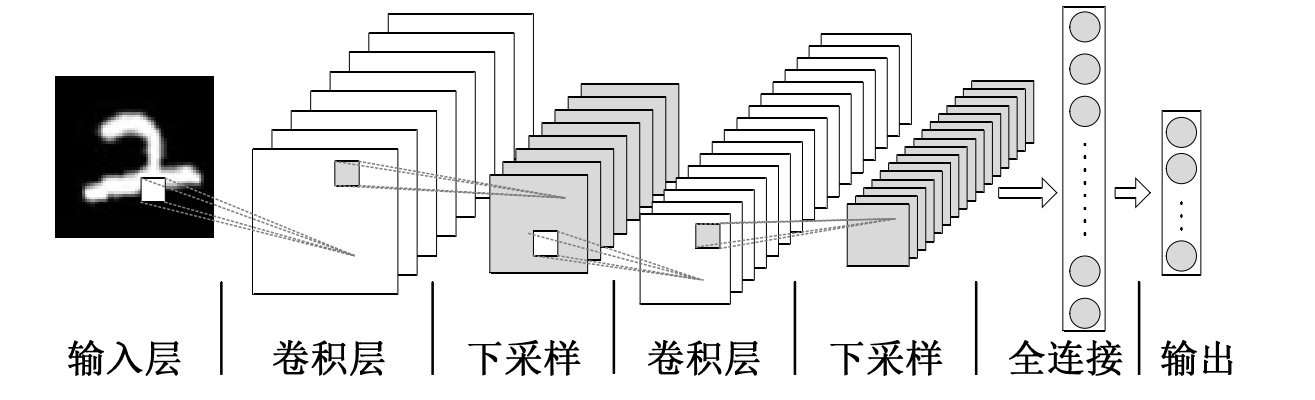
\includegraphics[width=.8\linewidth]{img/CNN.png}
\end{figure}


\subsection{生成对抗网络}

生成对抗网络(GAN)是另一种在图像处理中广泛应用的AI算法。GAN由两部分组成:生成器和判别器,它们一起形成了一个对抗的游戏。

\begin{itemize}
    \item 生成器:生成器的任务是生成尽可能真实的图像。它接收一个随机的噪声向量作为输入,通过一系列的反卷积和上采样操作,生成一个与真实图像相同大小的图像。生成器的目标是尽可能地欺骗判别器,使判别器无法区分生成的图像是真实的还是人工生成的。
    \item 判别器:判别器的任务是判断一个图像是真实的还是由生成器生成的。它接收一个图像作为输入,通过一系列的卷积和下采样操作,输出一个概率值,表示这个图像是真实的概率。判别器的目标是尽可能地识别出生成器生成的图像。
\end{itemize}

通过这种对抗的方式,GAN可以生成非常逼真的图像。例如生成新的人脸图像,这些图像非常逼真,以至于人类很难区分它们是真实的还是人工生成的。

\section{AI在图像处理中的应用}

\subsection{图像分类}

图像分类是AI在图像处理中的基础应用之一。图像分类一般是一个监督学习任务,它需要一个带有标签的图像数据集进行训练。例如可以使用CNN来训练一个模型,使其能够识别图像中的猫、狗、车、人等对象。

在训练过程中,CNN模型会自动学习图像的特征,并通过这些特征来区分不同的类别。例如,对于猫和狗的分类,CNN会学习到猫的耳朵通常是尖的,而狗的耳朵通常是圆的;猫的眼睛通常是狭长的,而狗的眼睛通常是圆的等特征。

\subsection{图像分割}

图像分割是将图像分割成多个区域,每个区域代表一个独立的对象。这是一个更复杂的任务,因为它不仅需要识别图像中的对象,还需要确定对象的边界。

最常见的图像分割方法是语义分割。我们可以使用CNN来进行语义分割,该技术可以将图像中的每个像素都分类到一个特定的类别,如人、车、树等。这需要一个带有像素级标签的图像数据集进行训练。

在训练过程中,CNN模型会自动学习像素的特征,并通过这些特征来区分不同的类别。例如,对于人和车的分割,CNN会学习到人的皮肤通常是平滑的,而车的表面通常是硬的;人的形状通常是垂直的,而车的形状通常是水平的等特征。

\begin{figure}[htbp]
    \centering
    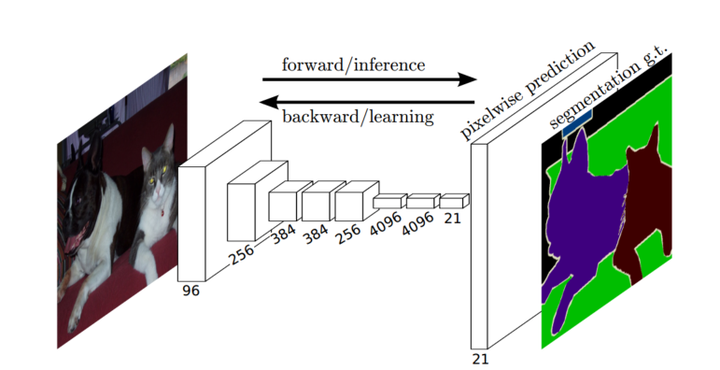
\includegraphics[width=.5\linewidth]{img/FCN.png}
\end{figure}

\subsection{图像生成}

图像生成是使用AI生成新的图像。图像生成一般是一个无监督学习任务,因为它不需要任何标签,只需要一个大量的图像数据集。

最常见的图像生成方法是生成对抗网络(GAN)。在训练过程中,生成器会尽量生成逼真的图像,而判别器会尽量识别出这些图像是人工生成的。通过这种对抗的方式,GAN模型可以不断提高生成图像的质量。例如对于人脸生成,GAN会学习到人的眼睛通常是对称的,鼻子通常在眼睛的中间,嘴巴通常在鼻子的下面等特征。

\begin{figure}[htbp]
    \centering
    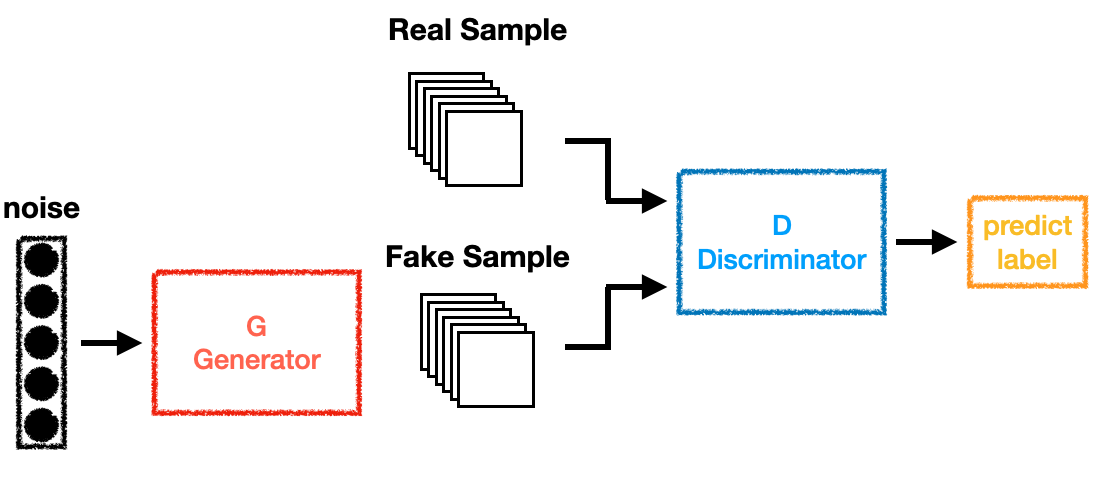
\includegraphics[width=.5\linewidth]{img/GAN.png}
\end{figure}

\section{为什么AI方法比传统方法效果好}

\paragraph{数据驱动}
深度学习是一种数据驱动的方法,它能够从大量的标注数据中学习和抽象出有用的特征。这与传统的计算机视觉方法(通常需要手动设计和选择特征)形成鲜明对比。随着可用数据量的增加,深度学习模型的性能通常会得到提升。

\paragraph{端到端学习}
深度学习模型可以直接从原始图像数据中学习到任务相关的表示,而无需手动设计特征提取器。这种端到端的学习方式使得模型可以在整个过程中进行优化,从而达到更好的性能。

\paragraph{模型容量}
深度学习模型通常具有很高的模型容量,这意味着它们可以表示和学习非常复杂的函数。这使得深度学习模型能够处理复杂的视觉任务,如物体检测、语义分割等。

\paragraph{泛化能力}
由于深度学习模型的能力在于学习数据的内在规律和结构,因此它们通常具有良好的泛化能力,即使在未见过的数据上也能表现出较好的性能。

\paragraph{硬件加速}
深度学习模型的训练和推理可以通过现代GPU进行高效的并行计算,大大加速了计算速度,使得在大规模数据上的训练成为可能。

\section{未来展望}
随着AI技术的发展,图像处理中会看到更多的创新应用。例如更精确的医疗影像分析帮助提高疾病的诊断准确率,更精确的车辆和行人检测技术助力自动驾驶技术的发展。

同时,AI在图像处理中的应用也带来了一些挑战。例如隐私问题,因为AI可以用来识别人脸和其他个人信息。此外,AI生成的图像可能会被用于制造深度伪造,这可能会对社会造成不利影响。

总的来说,AI在图像处理中的应用带来了巨大的机会和挑战,其背后的原理包括深度学习和生成对抗网络等复杂的算法。同时,我们也需要进一步研究和发展,以解决隐私、深度伪造等挑战,并继续推动AI在图像处理中的应用。

\end{document}
